\documentclass[journal,12pt,twocolumn]{IEEEtran}
\usepackage{setspace}
\usepackage{gensymb}
\usepackage{xcolor}
\usepackage{caption}
\singlespacing
\usepackage{siunitx}
\usepackage[cmex10]{amsmath}
\usepackage{mathtools}
\usepackage{hyperref}
\usepackage{amsthm}
\usepackage{mathrsfs}
\usepackage{txfonts}
\usepackage{stfloats}
\usepackage{cite}
\usepackage{cases}
\usepackage{subfig}
\usepackage{longtable}
\usepackage{multirow}
\usepackage{enumitem}
\usepackage{mathtools}
\usepackage{listings}
\usepackage{tikz}
\usetikzlibrary{shapes,arrows,positioning}
\usepackage{circuitikz}
\let\vec\mathbf
\DeclareMathOperator*{\Res}{Res}
\renewcommand\thesection{\arabic{section}}
\renewcommand\thesubsection{\thesection.\arabic{subsection}}
\renewcommand\thesubsubsection{\thesubsection.\arabic{subsubsection}}

\renewcommand\thesectiondis{\arabic{section}}
\renewcommand\thesubsectiondis{\thesectiondis.\arabic{subsection}}
\renewcommand\thesubsubsectiondis{\thesubsectiondis.\arabic{subsubsection}}
\hyphenation{op-tical net-works semi-conduc-tor}

\lstset{
language=Python,
frame=single, 
breaklines=true,
columns=fullflexible
}
\begin{document}
\theoremstyle{definition}
\newtheorem{theorem}{Theorem}[section]
\newtheorem{problem}{Problem}
\newtheorem{proposition}{Proposition}[section]
\newtheorem{lemma}{Lemma}[section]
\newtheorem{corollary}[theorem]{Corollary}
\newtheorem{example}{Example}[section]
\newtheorem{definition}{Definition}[section]
\newcommand{\BEQA}{\begin{eqnarray}}
        \newcommand{\EEQA}{\end{eqnarray}}
\newcommand{\define}{\stackrel{\triangle}{=}}
\newcommand{\myvec}[1]{\ensuremath{\begin{pmatrix}#1\end{pmatrix}}}
\newcommand{\mydet}[1]{\ensuremath{\begin{vmatrix}#1\end{vmatrix}}}

\bibliographystyle{IEEEtran}
\providecommand{\nCr}[2]{\,^{#1}C_{#2}} % nCr
\providecommand{\nPr}[2]{\,^{#1}P_{#2}} % nPr
\providecommand{\mbf}{\mathbf}
\providecommand{\pr}[1]{\ensuremath{\Pr\left(#1\right)}}
\providecommand{\qfunc}[1]{\ensuremath{Q\left(#1\right)}}
\providecommand{\sbrak}[1]{\ensuremath{{}\left[#1\right]}}
\providecommand{\lsbrak}[1]{\ensuremath{{}\left[#1\right.}}
\providecommand{\rsbrak}[1]{\ensuremath{{}\left.#1\right]}}
\providecommand{\brak}[1]{\ensuremath{\left(#1\right)}}
\providecommand{\lbrak}[1]{\ensuremath{\left(#1\right.}}
\providecommand{\rbrak}[1]{\ensuremath{\left.#1\right)}}
\providecommand{\cbrak}[1]{\ensuremath{\left\{#1\right\}}}
\providecommand{\lcbrak}[1]{\ensuremath{\left\{#1\right.}}
\providecommand{\rcbrak}[1]{\ensuremath{\left.#1\right\}}}
\theoremstyle{remark}
\newtheorem{rem}{Remark}
\newcommand{\sgn}{\mathop{\mathrm{sgn}}}
\newcommand{\rect}{\mathop{\mathrm{rect}}}
\newcommand{\sinc}{\mathop{\mathrm{sinc}}}
\providecommand{\abs}[1]{\left\vert#1\right\vert}
\providecommand{\res}[1]{\Res\displaylimits_{#1}}
\providecommand{\norm}[1]{\lVert#1\rVert}
\providecommand{\mtx}[1]{\mathbf{#1}}
\providecommand{\mean}[1]{E\left[ #1 \right]}
\providecommand{\fourier}{\overset{\mathcal{F}}{ \rightleftharpoons}}
\providecommand{\ztrans}{\overset{\mathcal{Z}}{ \rightleftharpoons}}
\providecommand{\system}[1]{\overset{\mathcal{#1}}{ \longleftrightarrow}}
\newcommand{\solution}{\noindent \textbf{Solution: }}
\providecommand{\dec}[2]{\ensuremath{\overset{#1}{\underset{#2}{\gtrless}}}}
\let\StandardTheFigure\thefigure
\def\putbox#1#2#3{\makebox[0in][l]{\makebox[#1][l]{}\raisebox{\baselineskip}[0in][0in]{\raisebox{#2}[0in][0in]{#3}}}}
\def\rightbox#1{\makebox[0in][r]{#1}}
\def\centbox#1{\makebox[0in]{#1}}
\def\topbox#1{\raisebox{-\baselineskip}[0in][0in]{#1}}
\def\midbox#1{\raisebox{-0.5\baselineskip}[0in][0in]{#1}}

\vspace{3cm}
\title{\LaTeX\ 11.10.1.7}
\author{Lokesh Surana}
\maketitle
\section*{Class 11, Exercse 10.1}

Q7. $\angle{PQR} = 100\degree$, where $\vec{P}, \vec{Q}$ and $\vec{R}$ are points on a circle with centre $\vec{O}$. Find $\angle{OPR}$

\solution 
Let, we have a unit circle with center at origin, i.e. $\vec{O} = \myvec{0\\0}$, and radius $r = 1$.
The points $\vec{P}, \vec{Q}$ and $\vec{R}$ are on the circle with center $\vec{O}$ and radius $r = 1$, such as
\begin{align}
    \vec{P} &= \myvec{\cos160\degree\\\sin160\degree} \\
    \vec{Q} &= \myvec{\cos\theta\\\sin\theta}  \\
    \vec{R} &= \myvec{\cos0\degree \\ \sin0\degree} = \myvec{1 \\ 0} \\
    \implies \vec{PQ} &= \vec{Q} - \vec{P} = \myvec{\cos\theta - \cos160\degree \\ \sin\theta - \sin160\degree} \\
    \implies \vec{QR} &= \vec{R} - \vec{Q} = \myvec{1 - \cos\theta \\ 0 - \sin\theta} 
\end{align}

As per given condition, we have
\begin{align}
    \angle{PQR} &= 100\degree 
    \label{eq:1} \implies \cos100\degree &= \frac{\vec{PQ}^\top \vec{QR}}{\norm{\vec{PQ}} \norm{\vec{QR}}} \\
\end{align}

\begin{align}
    \label{eq:2}   \norm{\vec{PQ}} &= \sqrt{\brak{\cos\theta - \cos160\degree}^2 + \brak{\sin\theta - \sin160\degree}^2} \\
    \label{eq:3}    \norm{\vec{QR}} &= \sqrt{\brak{1 - \cos\theta}^2 + \brak{0 - \sin\theta}^2} \\
    \label{eq:4}    \vec{PQ}^\top \vec{QR} &= -1 + \cos\theta + \cos{160\degree - \theta}
\end{align}

Using \eqref{eq:1}, \eqref{eq:2}, \eqref{eq:3} and \eqref{eq:4}, we get
\begin{align}
    \theta &= 32.31\degree\\
    \vec{Q} &= \myvec{\cos32.31\degree \\ \sin32.31\degree} = \myvec{0.999 \\ 0.032}   
\end{align}

\begin{figure}[!htb]
    \centering
    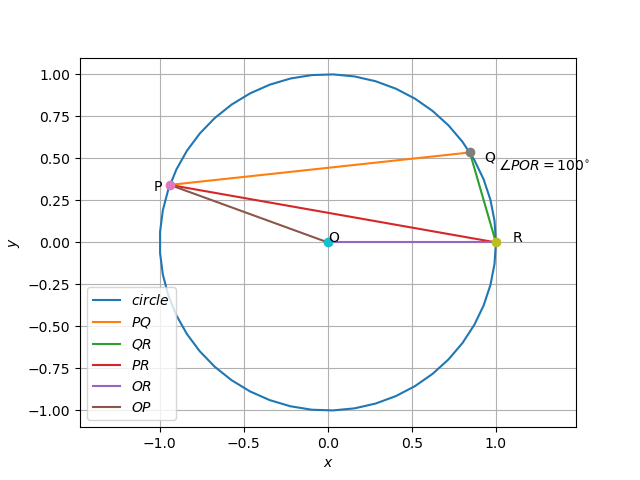
\includegraphics[width=\columnwidth]{figs/circle.png}
    \caption{circle}
    \label{fig:circle}
\end{figure}

Now, we'll find the $\angle{OPR}$,
\begin{align}
    \vec{OP} &= \vec{P} - \vec{O} = \myvec{\cos160\degree - 0 \\ \sin160\degree - 0} = \myvec{\cos160\degree \\ \sin160\degree} \\
    \vec{OR} &= \vec{R} - \vec{O} = \myvec{1 - 0 \\ 0 - 0} = \myvec{1 \\ 0} \\
    \implies \angle{OPR} &= \arccos\brak{\frac{\vec{OP}^\top \vec{OR}}{\norm{\vec{OP}} \norm{\vec{OR}}}} \\
    &= \arccos\brak{\frac{\cos160\degree + 1}{\sqrt{2}}} \\
    &= 20.87\degree
\end{align}

\end{document}